\documentclass[submit]{../harvardml}

\course{CS1810-S25}
\assignment{Assignment \#3}
\duedate{11:59pm EST, March 14th, 2025}

\usepackage{../common}
\usepackage[OT1]{fontenc}
\usepackage[colorlinks,citecolor=blue,urlcolor=blue]{hyperref}
\usepackage{graphicx}
\usepackage{amsmath}
\usepackage{amssymb}
\usepackage{framed}
\usepackage{color}
\usepackage{listings}
\usepackage{enumitem}
\usepackage{float}
\usepackage{comment}

%%%%%%%%%%%%%%%%%%%%%%%%%%%%%%%%%%%%%%%%%%%
%% Solution environment
\usepackage{xcolor}
\newenvironment{answer}{
    \vspace{2mm}
    \color{blue}\noindent\textbf{Solution}:
}{}
%%%%%%%%%%%%%%%%%%%%%%%%%%%%%%%%%%%%%%%%%%%

% \excludecomment{solution} % UNCOMMENT TO HIDE SOLUTIONS

% Student answer environment (used for answer templates)
% \newenvironment{answer}
%   {\section*{Solution}}
% {}

\DeclareMathOperator*{\mean}{\mathbb{E}}

\lstset{
  language=Python,
  basicstyle=\ttfamily,
  keywordstyle=\color{blue}\bfseries,
  commentstyle=\color{red},
  stringstyle=\color{green},
  frame=single,
  showstringspaces=false,
}

\definecolor{verbgray}{gray}{0.9}

\lstnewenvironment{csv}{%
  \lstset{backgroundcolor=\color{verbgray},
  frame=single,
  framerule=0pt,
  basicstyle=\ttfamily,
  columns=fullflexible}}{}

\begin{document}

\begin{center}
  {\Large Homework 3: Bayesian Methods and Neural Networks}\\
\end{center}

\subsection*{Introduction}

This homework is about Bayesian methods and neural networks.

\begin{enumerate}
  \item You'll explore the Bayesian paradigm and compare it with the frequentist paradigm for the Beta-Binomial conjugate pair.
  \item You'll derive the backpropagation algorithm for a single-hidden-layer neural network for the binary classification task.
  \item You'll write some code using the PyTorch library for an image classification task.
  \item You'll consider the opportunities and limitations of ML applications and learn to anticipate possible exploits of these systems.
\end{enumerate}

As always, please start early and come to office hours with questions!

\subsection*{Resources and Submission Instructions}
You may want to consider the lecture notes from Feb 18th to 27th (weeks 4 and 5).

Please type your solutions after the corresponding problems using this
\LaTeX\ template, and start each problem on a new page.

Please submit the \textbf{writeup PDF to the Gradescope assignment `HW3'}. Remember to assign pages for each question.  \textbf{You must include your plots in your writeup PDF. } The supplemental files will only be checked in special cases, e.g. honor code issues, etc.

Please submit your \textbf{\LaTeX\ file and code files to the Gradescope assignment `HW3 - Supplemental'}. \\


\newpage

%%%%%%%%%%%%%%%%%%%%%%%%%%%%%%%%%%%%%%%%%%%%%
% Problem 1
%%%%%%%%%%%%%%%%%%%%%%%%%%%%%%%%%%%%%%%%%%%%%

\begin{problem}[Connecting Bayesian and Frequentist Approaches, 40 pts]

In this question, we will gain practice with Bayesian modeling and
compare it with the frequentist paradigm.
In class, we discussed \emph{Normal-Normal conjugacy.} Now
we will turn to \emph{Beta-Binomial conjugacy.} This model can be
visualized in the following way.
You observe a fixed number \(N\) of coin flips (either
heads or tails) of which \(Y\) (a random variable) are heads. You assume that these are
drawn by flipping a coin with an unknown probability \(\theta\) of
landing heads. That is, we choose a \textbf{Binomial likelihood}
\(Y \sim \mathrm{Bin}(N, \theta)\). The PMF of this distribution is
given by

\[
  p(Y=y) = {N \choose y} \theta^{y} (1-\theta)^{N-y}.
\]

\begin{enumerate}
  \item[1.]
    \textbf{Frequentist paradigm and MLE.} The (log) likelihood is all we
    need for frequentist inference. Derive the MLE estimate for \(\theta\)
    given the observations \(Y = y\). That is, find
    \[\arg \max_{\theta} \log p(Y = y \mid \theta).\]

  \item[2.]
    \textbf{Beta-Binomial conjugacy.} Under the Bayesian paradigm, we must specify a
    prior distribution for the unknown parameter \(\theta\). We choose a \textbf{Beta prior}
    \(\theta \sim \mathrm{Beta}(\alpha, \beta)\). The PDF of this
    distribution is given by

    \[
      p(\theta) \propto \theta^{\alpha - 1} (1-\theta)^{\beta - 1}.
    \]

    When the prior and posterior belong to the same distribution family, we
    call the prior-and-likelihood pair a \textbf{conjugate pair.}

    For the rest of the problem, feel free to cite that the mean of the \(\mathrm{Beta}(\alpha, \beta)\) distribution is
    \[\mean[\theta] = \frac{\alpha}{\alpha+\beta},\]
    the mode is
    \[\arg\max_\theta p(\theta) = \frac{\alpha-1}{\alpha+\beta-2},\]
    and the variance is
    \[
      \mathrm{Var}(\theta) = \frac{\alpha \beta}{(\alpha + \beta)^2 (\alpha + \beta + 1)}.
    \]

    \begin{enumerate}
      \item
            Qualitatively speaking, what does the $\mathrm{Beta}(\alpha, \beta)$ distribution look like for different $\alpha$ and $\beta$? You can either plot this yourself or see \href{https://en.wikipedia.org/wiki/Beta_distribution}{its Wikipedia page}. What distribution does $\mathrm{Beta}(1, 1)$ correspond to?

      \item
            Show that the posterior
            \(p(\theta \mid Y=y)\) is indeed Beta and derive its parameters. This proves that a Beta prior and a Binomial likelihood form a conjugate pair; in other words, the Beta distribution is a \textbf{conjugate prior} for the Binomial distribution.

            \textbf{Hint} (for convenience in calculation): Do you need to calculate the normalizing constant?
    \end{enumerate}
\end{enumerate}
\end{problem}

\newpage

\begin{framed}
  \begin{enumerate}
    \item[3.]
      \textbf{Posterior mean and mode.} Often we wish to work with just a
      single point estimate of the posterior. Two commonly used point
      estimates are the \emph{posterior mean} and the \emph{posterior mode}
      (a.k.a. the maximum a posteriori (MAP) estimate).

      \begin{enumerate}
        \item
              Discuss the advantages and disadvantages of using posterior point
              estimates. Which of these are relevant for our Beta-Binomial conjugate pair?

        \item
              Using your results from part 2, write down

              \begin{enumerate}
                \item the posterior mean estimate \(\theta_{\text{post mean}} = \mean [\theta \mid Y = y]\),
                \item the posterior MAP estimate \(\theta_{\text{MAP}}=\arg \max_{\theta}p(\theta \mid Y=y)\),
                \item and the posterior variance $\mathrm{Var}(\theta \mid Y = y) = \mean[\theta^2 \mid Y = y] - (\mean[\theta \mid Y = y])^2$.
              \end{enumerate}

              \textbf{Hint}: Do you need to rederive anything? (This exercise should illustrate the power of conjugate priors!)

      \end{enumerate}

    \item[4.]
      \textbf{Prior-posterior connections.}

      \begin{enumerate}
        \item
              Explain in your own words how \(\alpha\) and \(\beta\) affect the
              MAP estimate. How would you set \(\alpha\) and \(\beta\) to reflect
              a prior belief that the coin is fair (i.e.~shows heads and tails
              with equal probability)? (Be careful that your answer does \emph{not} give high probability to an ``always heads'' coin or ``always tails'' coin!)

        \item Now let's analyze the variances of our prior and posterior distributions. Consider the case when $\alpha = \beta$. (If you'd enjoy it, consider the general case for better understanding.) Please write at most two sentences per point.
              \begin{enumerate}
                \item How does the variance of the prior relate to the variance of the posterior?
                \item How might you use the prior variance to encode a stronger or weaker prior belief?
                \item How does the posterior variance change as we observe more samples $n$?
              \end{enumerate}
      \end{enumerate}

    \item[5.]
      \textbf{Analysis and connection to frequentism.}

      \begin{enumerate}
        \item
              Write a loss function \(\ell(\theta) \in \mathbb{R}\) in terms of
              \(\theta, y, n, \alpha, \beta\) such that minimizing \(\ell\) is
              equivalent to calculating the MAP estimate,
              i.e.~\(\theta_{\text{MAP}} = \arg \min_{\theta} \ell(\theta)\). Your
              function should be a sum of:
              \begin{enumerate}
                \item a mean-squared-error term (which should loosely resemble $(y - \hat y)^2$)
                \item a
                      regularization term \(g(\theta) = - a \theta + b \theta^{2}\) for some $a, b$.
              \end{enumerate}

              Can you interpret the regularization term?

              \textbf{Hint}: Work backwards from part 1 to derive the MSE term and from the MAP in part 2 to get the regularization term. Watch out for the signs! For the interpretation, complete the square and then compare your expression with the prior mode in part 2.
        \item
              What happens to both $\theta_{\text{post mean}}$ and $\theta_{\text{MAP}}$ as \(n \to \infty\)? Compare this to the MLE estimate.
              (Remember to account for the change in \(y\).)
      \end{enumerate}

  \end{enumerate}

\end{framed}

\begin{answer}
  \begin{enumerate}
    \item[1.]
      Answer:
      \[
        \arg \max_{\theta} \log p(Y = y \mid \theta) = \frac{y}{N}
      \]
      Derivation:\\

      We are given our likelihoods since it is just the PMF of the binomial distribution $Y \sim Bin(N, \theta)$. Thus, since $\log$ is a monotonically increasing function, we can find the MLE from the log likelihood:

    \begin{align*}
        \log L(\theta) &= \log \binom{N}{y} + \log \theta^{y} + \log ((1-\theta)^{N-y}) \\
        &= \log\binom{N}{y} + y\log \theta + (N-y) \log(1-\theta)
    \end{align*}

    From the second derivative, we can see that this function is concave. Thus, if we take the first derivative of the log likelihood, setting it to 0 will allow us to find a maximum.

    \[
    \frac{dL(\theta)}{d\theta} = \frac{y}{\theta} - \frac{N-y}{1-\theta}
    \]

    Setting this equal to 0, we can solve for $\theta$ for the maximum.

    \[
    0 = \frac{y}{\theta} - \frac{N-y}{1-\theta}
    \]
    \[
    \frac{y}{\theta} =\frac{N-y}{1-\theta}
    \]
    \[
    N\theta - y\theta = y - y\theta
    \]
    \[
    \theta = \frac{y}{N}
    \]

    \item[2.]
      \begin{enumerate}
        \item
        From the Wikipedia, we can see that increasing $\alpha$ results in a left skew of the distribution while an increasing $\beta$ results in a right skew. When $\alpha = \beta > 1$, the distribution seems to have a lot of density in the center, but when $\alpha < 1$ and $\beta < 1$, the distribution becomes convex. The distribution of Beta$(1, 1)$ corresponds to a Unif$(0,1)$ distribution.

        \item

              Parameters:
              \[
                \alpha' = \alpha + y
              \]

              \[
                \beta' = \beta + N - y
              \]

              Derivation: \\

              We can use Bayes' rule, considering proportions instead of exact numbers since we know that the Beta PDF has a constant of proportionality.

              \begin{align*}
                  p(\theta | Y=y) &\propto p(Y=y | \theta)p(\theta) \\
                  &\propto \left[\binom{N}{y}\theta^y (1-\theta)^{N-y}\right]\left[\theta^{\alpha-1}(1-\theta)^{\beta - 1}\right] \\
                  &\propto \theta^{\alpha + y - 1}(1-\theta)^{\beta + N - y - 1}
                  \\
                  &= \frac{1}{c}\theta^{\alpha + y - 1}(1-\theta)^{\beta + N - y - 1}
              \end{align*}

              for some $c$ such that
              \[
              \int_{0}^1 \frac{1}{c}\theta^{\alpha + y - 1}(1-\theta)^{\beta + N - y - 1} = 1
              \]

              Thus, we can see that
              \[
              \theta | Y=y \sim Beta(\alpha + y, \beta + N - y)
              \]

      \end{enumerate}

    \item[3.]

      \begin{enumerate}
        \item
        Since our point estimates are for the posterior distribution, we get to see different aspects of the posterior with single point values instead of needing the entire distribution sample. This is simpler and easier than taking multiple samples or performing calculations over the entire distribution. However, single points can be misleading. For example, the posterior mode (MAP) may be easily changing between similar datasets. Additionally, the posterior mean could fall into a low density ready if the distribution is skewed or even if the distribution is multimodal.

        \item
              \begin{align*}
                \theta_{\text{post mean}} = \mean [\theta \mid Y = y]     & = \frac{\alpha + y}{\alpha + \beta + N}\\
                \theta_{\text{MAP}} =\arg \max_{\theta}p(\theta \mid Y=y) & = \frac{\alpha + y -1}{\alpha + \beta + N - 2}\\
                \mathrm{Var}(\theta \mid Y = y)                           & = \frac{(\alpha + y)(\beta + N - y)}{(\alpha + \beta + N)^2(\alpha + \beta + N + 1)}
              \end{align*}

      \end{enumerate}

    \item[4.]

      \begin{enumerate}
        \item
         We can see the results of adjusting this from the MAP estimate since $y$ represents heads and $N$ represents heads and tails. We see that increasing $\alpha$ would result in a unfair coins with heads being more likely and increasing beta $\beta$ would do the same but for a more likely tails. If we would want to set a prior belief that the coin is fair, we set $\alpha = \beta \ge 1$. However, if $\alpha = \beta < 1$, we get an extremely unfair come that is nearly always heads or tails and not fair. In general, though, the larger $\alpha + \beta$ is, the stronger the belief we have of our prior.

        \item
              \begin{enumerate}
                \item
                Our prior variance when $\alpha = \beta$ is $\frac{1}{8\alpha + 4}$, which is proportional to $\alpha^{-1}$. This is the same in the posterior case, which makes sense since the larger our $\alpha$ or $\beta$, the stronger we believe in our prior/results, which reduces variance.

                \item Having a smaller variance for our prior encodes a stronger belief since we are more confident in what we are assigning it to be, which arises from a larger $\alpha$ or $\beta$. Similarly, a larger variance indicates less confidence which encodes a weaker prior belief.

                \item In our posterior variance, we have a $N^2$ term in the denominator and a $N$ term in the numerator, which is around proportional to $N^{-1}$. Thus, as we observe more samples $N$ the posterior variance should decrease.
              \end{enumerate}

      \end{enumerate}

    \item[5.]

      \begin{enumerate}
        \item
              MSE term:
              \[
                M = \frac{1}{2N}(y - N\theta)^2
              \]

              Regularization term:
              \[
                R = -(\alpha - 1)\theta + \frac{1}{2}(\alpha + \beta - 2)\theta^2
              \]

              Loss function, as a function of the MSE and regularization term:
              \[
                \ell(\theta)  = \frac{1}{2N}(y - N\theta)^2 - (\alpha - 1)\theta + \frac{1}{2}(\alpha + \beta - 2)\theta^2
              \]

              \textbf{MSE term derivation:}\\

            We want to connect the Bayesian and frequentist perspective. Thus, for us to minimize the loss, we would equivalently want to maximize the likelihood of $\theta$ given the data. In other words, we wish to find a $\theta$ such that $\theta=\theta_{MAP}$. Thus, we can frame finding the critical point parameter for loss as finding $\theta=\theta_{MAP}$.

            \[
            \theta_{MAP} =\frac{\alpha + y -1}{\alpha + \beta + N - 2} 
            \]

            so we can write

            \[
              \nabla \ell(\theta) =\theta({\alpha + \beta + N - 2}) - (\alpha + y -1) = 0
            \]

            Thus, to find the loss function $\ell(\theta)$, we can take the integral with respect to $\theta$ to get:

            \[
              \ell(\theta) = \frac{1}{2}(\alpha + \beta + N - 2)\theta^2 - (\alpha + y -1)\theta + C
            \]

            Recall our goal of finding a loss function as a sum of a mean-squared-error term and a regularization term $g(\theta)$. We can expand the expression toget

            \[
            \ell(\theta) = \frac{1}{2} \alpha \theta^2 + \frac{1}{2}\beta\theta^2 + \frac{1}{2}N\theta^2 - \theta^2 - \alpha\theta - y\theta + \theta + C
            \]

            We know our MSE term will be along the lines of $(y - \hat{y})^2$. From linearity of expectation, we know that our expected amount of heads is $N\cdot \theta$, so we wish to find some term

            \[
            k(y - N\theta)^2
            \]

            for some $k$. We can complete the square from our above expression, seeing that:

            \[
            \frac{1}{2}N\theta^2 - y\theta + \frac{y^2}{2N} = \frac{1}{2N}(N^2\theta^2 - 2yN\theta + y^2) = \frac{1}{2N}(y - N\theta)^2
            \]

            Since we take the derivative to find the minimal loss value and $C$ is a constant, we can set $C=\frac{y^2}{2N}$ since $N$ is fixed. Therefore, we can write our expression:

            \[
            \ell(\theta) = \frac{1}{2N}(y - N\theta)^2 - (\alpha - 1)\theta + \frac{1}{2}(\alpha + \beta - 2)\theta^2
            \]

            Therefore, we see that our expression is split into a MSE term and a regularization term.\\              
              

              \textbf{Regularization term derivation:}\\

              We can similarly derive our regularization term from the above expression:
            \[
                \ell(\theta) = \frac{1}{2N}(y - N\theta)^2 - (\alpha - 1)\theta + \frac{1}{2}(\alpha + \beta - 2)\theta^2
            \]
              We wanted a term $g(\theta) = -a \theta + b \theta^2$. Thus we have

              \[
              a = \alpha - 1
              \]
              \[
              b = \frac{1}{2}(\alpha + \beta - 2)
              \]

              which result in the regularization term $g(\theta)$. \\

              \textbf{Regularization term interpretation:}\\

              Let us consider our regularization term

              \[
              g(\theta) = -(\alpha - 1)\theta + \frac{1}{2}(\alpha + \beta - 2)\theta^2
              \]

              We can complete the square. Let us first rewrite the expression with $c = \frac{1}{2}(\alpha + \beta - 2)$.

              \[
              c\theta^2 - (\alpha - 1)\theta
              \]
              \[
              c\left(\theta^2 - \frac{\alpha - 1}{c}\theta\right)
              \]
              Let us also write $d = \frac{\alpha - 1}{c}$ for sake of computation.
              \[
              = c(\theta^2 - d\theta)
              \]
              \[
              c\left(\theta^2-d\theta+\left(\frac{d}{2}\right)^2\right) - c\left(\frac{d}{2}\right)^2
              \]
              \[
              c\left(\theta - \frac{d}{2}\right)^2 - c\left(\frac{d}{2}\right)^2
              \]

              Substituting our expressions in, we get:

              \[
              g(\theta) = \frac{\alpha + \beta -2}{2}\left(\theta - \frac{\alpha - 1}{\alpha + \beta -2}\right)^2 - \frac{(\alpha - 1)^2}{2(\alpha + \beta -2)}
              \]

              Notice that this expression contains the mode of the prior.

              \[\arg\max_\theta p(\theta) = \frac{\alpha-1}{\alpha+\beta-2}\]

              \[
              g(\theta) = \frac{\alpha + \beta -2}{2}\left(\theta - arg\max_\theta p(\theta)\right)^2 - \frac{(\alpha - 1)^2}{2(\alpha + \beta -2)}
              \]

              Thus, we can interpret our regularization term to penalize $\theta$'s that are different from our prior mode (since the other subtracted value is just a constant, it does not affect our loss minimization). Therefore, our MSE penalizes distance from our posterior MLE while our regularization term penalizes distance from our prior mode.

        \item As the total flips $n \to \infty$, we know that the number of heads $y$ also increases proportionally. The values $\alpha$ + $\beta$ are constant, so $\theta_{\text{post mean}} \to \frac{y}{N}$ and $\theta_{MAP} \to \frac{y}{N}$ as the number of flips increases. This is the same as the MLE estimate we found above.

      \end{enumerate}

  \end{enumerate}
\end{answer}


\newpage

%%%%%%%%%%%%%%%%%%%%%%%%%%%%%%%%%%%%%%%%%%%%%
% Problem 2
%%%%%%%%%%%%%%%%%%%%%%%%%%%%%%%%%%%%%%%%%%%%%

\begin{problem}[Neural Networks, 20 pts]

In this problem, we will take a closer look at how gradients are calculated for backpropagation with a simple multi-layer perceptron (MLP). The MLP will consist of a first fully connected layer with a sigmoid activation, followed by a one-dimensional, second fully connected layer with a sigmoid activation to get a prediction for a binary classification problem. We use non-linear activation functions as the composition of linear functions is linear. Assume bias has not been merged. Let:
\begin{itemize}
  \item $\bold{W}_1$ be the weights of the first layer, $\bold{b}_1$ be the bias of the first layer.
  \item $\bold{W}_2$ be the weights of the second layer, $\bold{b}_2$ be the bias of the second layer.
\end{itemize}

The described architecture can be written mathematically as: $$\hat{y} = \sigma(\bold{W}_2 \left[\sigma \left(\bold{W}_1 \bold{x} + \bold{b}_1\right)\right] + \bold{b}_2)$$

where $\hat{y}$ is a scalar output of the net when passing in the single datapoint $\bold{x}$ (represented as a column vector), the additions are element wise additions, and the sigmoid is an element wise sigmoid.

\begin{enumerate}
  \item Let:
        \begin{itemize}
          \item $N$ be the number of datapoints we have
          \item $M$ be the dimensionality of the data
          \item $H$ be the size of the hidden dimension of the first layer. Here, hidden dimension is used to describe the dimension of the resulting value after going through the layer. Based on the problem description, the hidden dimension of the second layer should be 1.
        \end{itemize}

        Write out the dimensionality of each of the parameters, and of the intermediate variables:

        \begin{align*}
          \bold{a}_1 & = \bold{W}_1 \bold{x} + \bold{b}_1,
                     & \bold{z}_1 = \sigma(\bold{a}_1)       \\
          a_2        & = \bold{W}_2 \bold{z}_1 + \bold{b}_2,
                     & \hat{y} = z_2 = \sigma(a_2)
        \end{align*}

        and make sure they work with the mathematical operations described above. Examining shapes is one of the key ways to debug your code, and can be done using .shape after any numpy array.

  \item  We will derive the gradients for each of the parameters, which can then be used along with gradient descent to find weights that improve our model's performance. For this question, assume there is only one datapoint $\bold{x}$, and that our loss is $L = -(y \log (\hat{y}) + (1 - y) \log (1 - \hat{y}))$. For all questions, the chain rule will be useful.
        \begin{enumerate}
          \item Find $\frac{\partial L}{\partial b_2}$.

          \item Find $\frac{\partial L}{\partial W_2^h}$, where $W_2^h$ represents the $h$th element of $\bold{W}_2$.

          \item Find $\frac{\partial L}{\partial b_1^h}$, where $b_1^h$ represents the $h$th element of $\bold{b}_1$. (\textbf{Hint}: Note that only the $h$th element of $\bold{a}_1$ and $\bold{z}_1$ depend on $b_1^h$ - this should help you with how to use the chain rule.)

          \item Find $\frac{\partial L}{\partial W_1^{h, j}}$, where  $W_1^{h,j}$ represents the element in row $h$, column $j$ in $\bold{W}_1$.

        \end{enumerate}

\end{enumerate}

\end{problem}

\newpage

\begin{framed}
  \noindent\textbf{Problem 2} (cont.)\\
  \begin{enumerate}
    \setcounter{enumi}{2}

    \item  We now explore an example of forward-mode auto-differentiation. Consider the following
          equation:

          $$
            f(x_1, x_2) = \ln (\sin (x_1)) + x_1 \exp \{ x_2 \}
          $$

          This equation can be split up using intermediate variables $v_1, \dots, v_7$ as follows:

          \begin{align*}
            v_1         & = x_1            \\
            v_2         & = \sin (v_1)     \\
            v_3         & = \ln (v_2)      \\
            v_4         & = x_2            \\
            v_5         & = \exp \{ v_4 \} \\
            v_6         & = v_1v_5         \\
            v_7         & = v_3 + v_6      \\
            f(x_1, x_2) & = v_7
          \end{align*}

          Splitting up the equation like this is very similar to what an auto-differentiation
          library would do. From these equations we can construct a \textit{computational graph}
          where each node of the graph corresponds to an input, an intermediate variable, or
          the output.

          \begin{enumerate}
            \item Let $x_1 = \frac{\pi}{6}$ and $x_2 = 1$. Calculate the values of all the
                  intermediate variables $v_1, \dots v_7$ and $f(x_1,x_2)$.
            \item Calculate the derivative of
                  all of the intermediate variables $v_1, \dots, v_7$ and
                  $f$ with respect to $x_1$ evaluated
                  at $x_1 = \frac{\pi}{6}$ and $x_2 = 1$. Remember to write out the equations before evaluating, e.g.,
                  \[
                    \frac{\partial f(x)}{\partial x} = \frac{\partial f(x)}{\partial g(x)} \frac{\partial g(x)}{\partial x}.
                  \]
          \end{enumerate}
  \end{enumerate}
\end{framed}

\begin{answer}
  \begin{enumerate}
    \item \begin{itemize}
            \item $\bold{W}_1 : H\times M$
            \item $\bold{b}_1 : H \times 1$
            \item $\bold{W}_2 : 1\times H$
            \item $\bold{b}_2 : 1\times 1$
            \item $\bold{a}_1 : H\times 1$
            \item $\bold{z}_1 : H\times 1$
            \item $a_2 : 1\times 1$
            \item $\hat{y} : 1\times 1$
          \end{itemize}

    \item \begin{enumerate}
            \item
                  \begin{align*}
                    \frac {\partial L}{\partial b_2} & = \frac{\partial L}{\partial \hat{y}}\cdot \frac{\partial \hat{y}}{\partial a_2}\cdot\frac{\partial a_2}{\partial b_2} \\
                    &= \left(-\left(\frac{y}{\hat{y}}-\frac{1-y}{1-\hat{y}}\right)\right) \cdot (\hat{y}(1-\hat{y}))\cdot 1 \\
                    &= \boxed{\hat{y} - y}
                  \end{align*}

            \item
                  \begin{align*}
                    \frac {\partial L}{\partial W_2^h} & = \frac{\partial L}{\partial \hat{y}}\cdot \frac{\partial \hat{y}}{\partial a_2} \cdot \frac{\partial a_2}{\partial W_2^h} \\
                    &=\boxed{(\hat{y} - y)z_1^h}
                  \end{align*}

                  since we can write

                  \[
                  a_2 = W_2z_1 + b_2 = \sum_{i} W_2^iz_1^i + b_2
                  \]
                  \[
                  \frac{\partial a_2}{\partial W_2^h} = z_1^h
                  \]

                  so we substitute this above.

            \item
                  \begin{align*}
                    \frac {\partial L}{\partial b_1^h} & = \frac{\partial L}{\partial \hat{y}}\cdot \frac{\partial\hat{y}}{\partial a_2}\cdot \frac{\partial a_2}{\partial z_1^h} \cdot \frac{\partial z_1^h}{\partial a_1^h} \cdot \frac{\partial a_1^h}{\partial b_1^h} \\
                    &= \boxed{(\hat{y} - y)W_2^h(z_1^h(1-z_1^h))}
                  \end{align*}

                  using the hint and since we can write

                  \[
                  a_2 = W_2 z_1 + b_2 = \sum_{i}W_2^iz^i + b_2
                  \]

                  we can get the following:
                  \begin{align*}
                      \frac{\partial a_2}{\partial z_1^h} &= W_2^h \\
                      \frac{\partial z_1^h}{\partial a_1^h} &= z_1^h(1-z_1^h) \\
                      \frac{\partial a_1^h}{\partial b_1^h} &= 1
                  \end{align*}

            \item
                  \begin{align*}
                    \frac {\partial L}{\partial W_1^{h,j}} & = \frac{\partial L}{\partial \hat{y}}\cdot \frac{\partial\hat{y}}{\partial a_2}\cdot \frac{\partial a_2}{\partial z_1^h} \cdot \frac{\partial z_1^h}{\partial a_1^h} \cdot \frac{\partial a_1^h}{\partial W_1^{h,j}} \\
                    &= \boxed{(\hat{y} - y)W_2^h(z_1^h(1-z_1^h))x^j}
                  \end{align*}

                  since we can write

                  \[
                  a_1^h = \sum_{i}W^{h,i}x^i + b^h
                  \]
                  \[
                  \frac{\partial a_1^h}{\partial W_1^{h,j}} = x^j
                  \]

                  and the rest we have already found from previous derivations.
          \end{enumerate}

    \item

          \begin{enumerate}
            \item
                  \begin{align*}
                    v_1        & = \frac{\pi}{6}\\
                    v_2        & = \frac{1}{2}\\
                    v_3        & = \ln\left(\frac{1}{2}\right) \approx -0.6931471806\\
                    v_4        & = 1\\
                    v_5        & = e\\
                    v_6        & = \frac{\pi}{6}\cdot e\\
                    v_7        & = \ln\left(\frac{1}{2}\right) + \frac{\pi e}{6} \approx 0.7301418\\
                    f(x_1,x_2) & = \ln\left(\frac{1}{2}\right) + \frac{\pi e}{6}  \approx 0.7301418\\
                  \end{align*}

            \item
                  \begin{align*}
                    \frac{\partial v_1}{\partial x_1} & = \frac{\partial}{\partial x_1} x_1 = \boxed{1}\\
                    \frac{\partial v_2}{\partial x_1} & = \frac{\partial v_2}{\partial v_1}\cdot \frac{\partial v_1}{\partial x_1}\\
                    &=\cos(v_1)\rvert_{v_1=x_1=\frac{\pi}{6}}=\boxed{\frac{\sqrt{3}}{2}}\\
                    \frac{\partial v_3}{\partial x_1} & = \frac{\partial v_3}{\partial v_2}\cdot \frac{\partial v_2}{\partial v_1}\cdot \frac{\partial v_1}{\partial x_1}\\
                    &= \left. \frac{1}{v_2}\cos(v_1)\right|_{v_2=\sin(x_1),v_1=x_1=\pi/6} =\boxed{\sqrt{3}}\\
                    \frac{\partial v_4}{\partial x_1} & = \left. \frac{\partial}{\partial x_1} x_2 \right|_{x_2=1} = \boxed{0}\\
                    \frac{\partial v_5}{\partial x_1} & = \frac{\partial v_5}{\partial v_4} \cdot \frac{\partial v_4}{\partial x_1} = \left. e^{x_2}\cdot 0 \right|_{x_2=1}= \boxed{0}\\
                    \frac{\partial v_6}{\partial x_1} & = \frac{\partial v_6}{\partial v_1} \cdot \frac{\partial v_1}{\partial x_1} = \frac{\partial}{\partial v_1} v_1v_5 \cdot 1\\
                    &= v_5 \rvert_{v_5=e^{x_2},x_2=1} = \boxed{e \approx 2.718}\\
                    \frac{\partial v_7}{\partial x_1} & = \frac{\partial}{\partial x_1} (v_3 + v_6) = \frac{\partial v_3}{\partial x_1} + \frac{\partial v_6}{\partial x_1}\\
                    &= \boxed{\sqrt{3} + e \approx 4.450}\\
                    \frac{\partial f}{\partial x_1}   & = \frac{\partial v_7}{\partial x_1} = \boxed{\sqrt{3} + e \approx 4.450}
                  \end{align*}
          \end{enumerate}

  \end{enumerate}
\end{answer}


\newpage

%%%%%%%%%%%%%%%%%%%%%%%%%%%%%%%%%%%%%%%%%%%%%
% Problem 3
%%%%%%%%%%%%%%%%%%%%%%%%%%%%%%%%%%%%%%%%%%%%%

\begin{problem}[Modern Deep Learning Tools: PyTorch, 40 pts]

In this problem, you will learn how to use PyTorch. This machine learning library is massively popular and used heavily throughout industry and research.


\begin{enumerate}
  \item In \verb|homework3.ipynb| you will implement an MLP for image classification from scratch. Paste your code solutions below and include a final graph of your training progress. Also, submit your completed \verb|homework3.ipynb| file.
  \item Discuss what trends you see with your plot (train/test loss and train/test accuracy).

  \item \textbf{Out of Distribution (OOD) Analysis}: Now, let's evaluate the usefulness of the predictive uncertainties of our model for test data that are dissimilar to our training data. These test data points are called out of distribution (OOD) points. Report both the in and out distribution test accuracies of your model. In a couple of sentences, discuss what you notice about these accuracies.

  \item Now let us consider the implications of what we have seen.  First, just as in Homework 2, we want the predictive uncertainties from our models to help us distinguish in-distribution test data (test data that are similar to data on which we trained our model) and OOD test data.  Look at some examples in which the model expresses uncertainty about an in-distribution output and in which the model expresses uncertainty about an out-of-distribution output.  Characterize what you see.  In what ways are the uncertainties of the model useful, and in what ways are they not?  Do you think training multiple models and boostrapping, like you did in Homework 2, would help?  (You do not have to code anything, just discuss.)

  \item Suppose the postal service was going to use your model to help automatically sort mail by zipcodes (a real use of AI systems).  They want to make sure that their system is safe against adversarial attacks.  Let us suppose that the model is relatively safe against software attacks, that is, appropriate security is in place such that the adversary cannot simply change the weights of a deployed model without someone noticing (in practice, this would be an important element).  Three scenarios, however, are of concern to them:
        \begin{enumerate}
          \item Hardware attack: Suppose the adversary has access to the
                scanner used to take pictures of the envelopes.  How might
                they be able to change the outputs of the model to their
                desired ones?  What safeguards might be possible, and what
                are their benefits and limitations/drawbacks?
          \item Input attack: Suppose the adversary has access to the
                envelopes prior to scanning.  How might they be able to
                change the outputs of the model to their desired ones?
                What safeguards might be possible, and what are their
                benefits and limitations/drawbacks?
          \item Social Engineering attack: Suppose that the adversary
                has access to the teams that will be maintaining and
                retraining the model.  How might they be able to change the
                outputs of the model to their desired ones?  What safeguards
                might be possible, and what are their benefits and
                limitations/drawbacks?
        \end{enumerate}
        \textbf{In no more than 10 lines}, consider possible safeguards that might be implemented to the software, system integration, and work environment overall?  You may find
        it useful to explore how you can manipulate your model by
        changing inputs, etc. but no coding is required for this
        question.

\end{enumerate}

{\bfseries You will recieve no points for code not included below.}

{\bfseries You will recieve no points for code using built-in APIs from the \verb|torch.nn| library.}

\end{problem}


\begin{answer}

  \begin{enumerate}
    \item[1.]

      Plot:
      
      \begin{figure}[H]
        \centering
        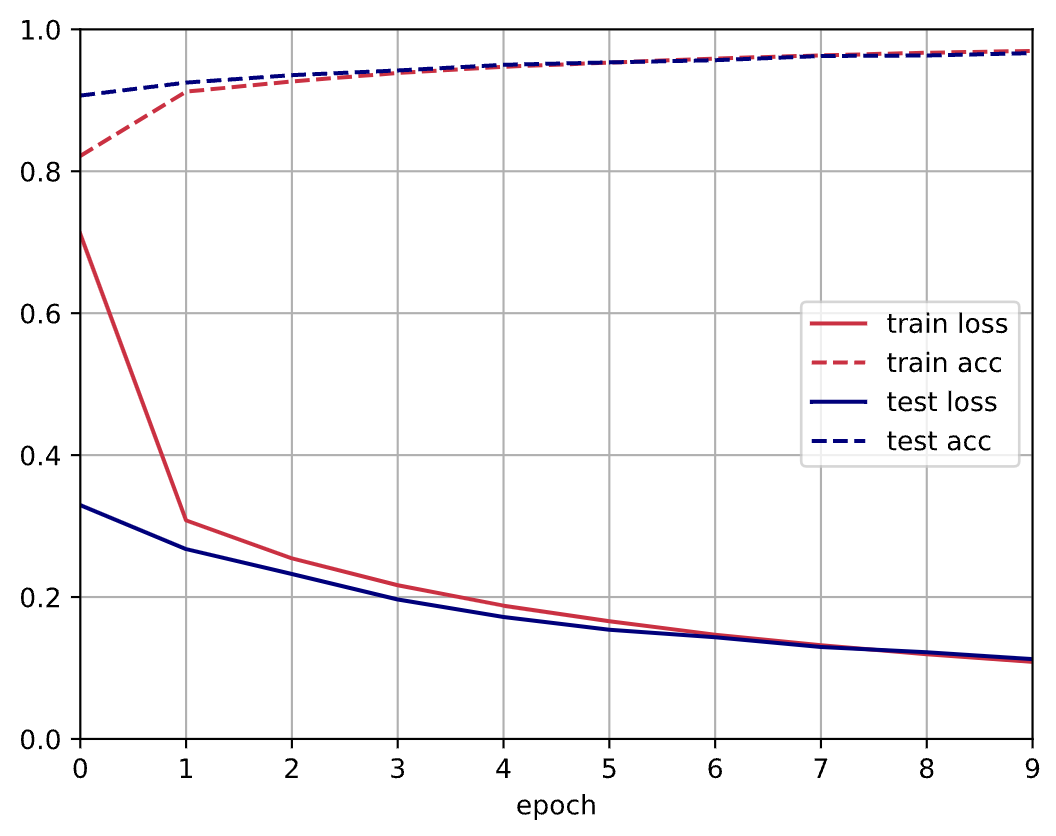
\includegraphics[width=0.5\linewidth]{nn_accuracy.png}
    \end{figure}

      Code:

      \begin{lstlisting}[language=Python]

n_inputs = 784 
n_hiddens = 256
n_outputs = 10

W1 = torch.nn.Parameter(0.01 * torch.randn(n_inputs, n_hiddens)) 
b1 = torch.nn.Parameter(torch.zeros(n_hiddens)) 
W2 = torch.nn.Parameter(0.01 * torch.randn(n_hiddens, n_outputs))
b2 = torch.nn.Parameter(torch.zeros(n_outputs))


def relu(x):
  return torch.clamp(x, min=0)


def softmax(x):
  exp_X = torch.exp(X)
  denom = torch.sum(exp_X, dim=1, keepdim=True)
  return exp_X / denom


def net(X):
  X = X.flatten(start_dim=1)
  H = relu(X @ W1 + b1)
  O = softmax(H @ W2 + b2)
  return O


def cross_entropy(y_hat, y):
  y_hat_y = y_hat[range(len(y_hat)), y]
  return -torch.log(y_hat_y)


def sgd(params, lr=0.1):
  with torch.no_grad():
    for w in params:
      w -= lr * w.grad
      w.grad.zero_()



def train(net, params, train_iter, loss_func=cross_entropy, updater=sgd):
  for _ in range epochs: # Seemingly undefined but it's in the instructions
    for X, y  in train_iter:
      y_hat = net(X)
      loss = loss_func(y_hat, y)
      total_loss = loss.mean()
      total_loss.backward()
      updater(params)


\end{lstlisting}

    \item[2.]
    The training loss begins very high but quickly decreases while the training accuracy increases. The test loss begins lower, which makes sense since it corresponds to measurements of the data presented after training and the accuracy also begins higher. However, the metrics for training and test converge quickly as the epochs grow, with the accuracy for both almost reaching 1.0 and loss reaching around 0.1. The NN seems to quickly fit from the 0th to 1st epoch and gradually improves through more iterations.

    \item[3.]

      Test Accuracy (In Distribution): \textbf{0.9963235294117647}

      Test Accuracy (Out of Distribution): \textbf{0.0}

      Discussion: The high test accuracy of the In Distribution data is very high, suggesting that the model has learned the patterns well from the training data. Its performance for familiar data indicates that it has fit to the training data. However, the extremely low Out of Distribution test accuracy (0.0) suggests that the model poorly generalizes to data that is not within the training. This makes sense since we only train on 1's and 6's and then our Out of Distribution data is just 3's, which the model would never have encountered before. As a result, the model likely only outputs 1 or 6 for all inputs, which would result in a worse accuracy than just guessing of 0.
      

    \item[4.]
    The uncertainty from the in distribution data is mostly between more similar looking digits. We can see from the confusion table, though, that the model performs quite well, but the overall uncertainty stems from the differences in what the image looks like (e.g. 1 vs 6). However, for out-of-distribution data the model could be very confident on an answer and just be wrong. For example, if it learns that the data is only 1's and 6's in training, it would likely not consider any of the other outputs as much. Thus, we given a 3, it would be very certain that the image is likely a 1 or 6 but be completely off. Thus, uncertainty is useful when we know the universe of data, but does not provide insight into model performance unless paired with other metrics (such as accuracy). Training multiple models and boostrapping would help for in-distribution uncertainty. However, for out-of-distribution test data, it would likely not help.
    

    \item[5.]
    Should we write in no more than 10 lines for all?
        

      \begin{enumerate}
        \item The adversary could affect how the images of the envelopes are presented. They could change the background of the envelope to be neon red or could blur the image by smearing the camera. Some safeguards are to train a the NN by adding noise or having different backgrounds in the training data. We could alert humans when any erroneous attacks are present for manual checking.
        \item If some envelopes are slightly altered so that the NN would interpret it (for example smudging numbers, making it look like 5 is 6), we could some envelopes be supervised by humans to check whether or not the NN is working properly or if there has been any tampering.
        \item The adversary could train a new model on different data to purposely malfunction on certain inputs (for example, all 1's are read as 5's). Some safeguards would be to check random data points in a dataset and verify the authenticity of any information used.
      \end{enumerate}


  \end{enumerate}

\end{answer}


%%%%%%%%%%%%%%%%%%%%%%%%%%%%%%%%%%%%%%%%%%%%%
% Name and Calibration
%%%%%%%%%%%%%%%%%%%%%%%%%%%%%%%%%%%%%%%%%%%%%
\newpage
\subsection*{Name: Charles Zhou} 

\subsection*{Collaborators and Resources}
Whom did you work with, and did you use any resources beyond cs181-textbook and your notes?

Davin Jeong

\end{document}
